\documentclass[namedreferences]{solarphysics}

\usepackage[hyperref,optionalrh,showbiblabels]{spr-sola-addons} % For Solar Physics 
%\usepackage[optionalrh]{spr-sola-addons} % For Solar Physics 
%\usepackage{epsfig}          % For eps figures, old commands
\usepackage{graphicx}        % For eps figures, newer & more powerfull
%\usepackage{courier}         % Change the \texttt command to courier style
%\usepackage{amssymb}        % useful mathematical symbols
\usepackage{color}           % For color text: \color command
\usepackage{breakurl}        % For breaking URLs easily trough lines
\def\UrlFont{\sf}            % define the fonts for the URLs

% General definitions
% please place your own definitions here and don't use \def but
% \newcommand{}{} or 
% \renewcommand{}{} if it is already defined in LaTeX

\newcommand{\BibTeX}{\textsc{Bib}\TeX}
\newcommand{\etal}{{\it et al.}}

% Definitions for equations
\renewcommand{\vec}[1]{{\mathbfit #1}}
\newcommand{\deriv}[2]{\frac{{\mathrm d} #1}{{\mathrm d} #2}}
\newcommand{\rmd}{ {\ \mathrm d} }
\newcommand{\uvec}[1]{ \hat{\mathbf #1} }
\newcommand{\pder}[2]{ \f{\partial #1}{\partial #2} }
\newcommand{\grad}{ {\bf \nabla } }
\newcommand{\curl}{ {\bf \nabla} \times}
\newcommand{\vol}{ {\mathcal V} }
\newcommand{\bndry}{ {\mathcal S} }
\newcommand{\dv}{~{\mathrm d}^3 x}
\newcommand{\da}{~{\mathrm d}^2 x}
\newcommand{\dl}{~{\mathrm d} l}
\newcommand{\dt}{~{\mathrm d}t}
\newcommand{\intv}{\int_{\vol}^{}}
\newcommand{\inta}{\int_{\bndry}^{}}
\newcommand{\avec}{ \vec A}
\newcommand{\ap}{ \vec A_p}

\newcommand{\bb}{\vec B}
\newcommand{\jj}{ \vec j}
\newcommand{\rr}{ \vec r}
\newcommand{\xx}{ \vec x}

% Definitions for the journal names
\newcommand{\adv}{    {\it Adv. Space Res.}} 
\newcommand{\annG}{   {\it Ann. Geophys.}} 
\newcommand{\aap}{    {\it Astron. Astrophys.}}
\newcommand{\aaps}{   {\it Astron. Astrophys. Suppl.}}
\newcommand{\aapr}{   {\it Astron. Astrophys. Rev.}}
\newcommand{\ag}{     {\it Ann. Geophys.}}
\newcommand{\aj}{     {\it Astron. J.}} 
\newcommand{\apj}{    {\it Astrophys. J.}}
\newcommand{\apjl}{   {\it Astrophys. J. Lett.}}
\newcommand{\apss}{   {\it Astrophys. Space Sci.}} 
\newcommand{\cjaa}{   {\it Chin. J. Astron. Astrophys.}} 
\newcommand{\gafd}{   {\it Geophys. Astrophys. Fluid Dyn.}}
\newcommand{\grl}{    {\it Geophys. Res. Lett.}}
\newcommand{\ijga}{   {\it Int. J. Geomagn. Aeron.}}
\newcommand{\jastp}{  {\it J. Atmos. Solar-Terr. Phys.}} 
\newcommand{\jgr}{    {\it J. Geophys. Res.}}
\newcommand{\mnras}{  {\it Mon. Not. Roy. Astron. Soc.}}
\newcommand{\nat}{    {\it Nature}}
\newcommand{\pasp}{   {\it Pub. Astron. Soc. Pac.}}
\newcommand{\pasj}{   {\it Pub. Astron. Soc. Japan}}
\newcommand{\pre}{    {\it Phys. Rev. E}}
\newcommand{\solphys}{{\it Solar Phys.}}
\newcommand{\sovast}{ {\it Soviet  Astron.}} 
\newcommand{\ssr}{    {\it Space Sci. Rev.}} 
\chardef\us=`\_

%%%%%%%%%%%%%%%%%%%%%%%%%%%%%%%%%%%%%%%%%%%%%%%%%%%%%%%%%%%%%%%%%%
\begin{document}

\begin{article}
\begin{opening}

\title{Article preparation guidelines\\ {\it Solar Physics}}

\author[addressref={aff1,aff2,aff3},corref,email={e-mail.a@mail.com}]{\inits{F.N.}\fnm{F. Name}~\lnm{Author-a}}%\sep
\author[addressref=aff1,email={e-mail.b@mail.com}]{\inits{F.}\fnm{Fisrt}~\lnm{Author-b}}%\sep
\author[corref,email={e-mail.c@mail.com}]{\inits{S.}\fnm{Second}~\lnm{Author-c}}%\sep
\author{\inits{T.}\fnm{Third}~\lnm{Author-x}}
%\author{\inits{}\fnm{}~\lnm{}\orcid{}}
%\author{P.~\surname{Author-a}$^{1}$\sep
%        E.~\surname{Author-b}$^{1}$\sep
%        M.~\surname{Author-c}$^{2}$      
%       }

%   \institute{$^{1}$ First affiliation
%                     email: \url{e.mail-a} email: \url{e.mail-b}\\ 
%              $^{2}$ Second affiliation
%                     email: \url{e.mail-c} \\
%             }
\address[id=aff1]{First very very very very very very very very very
 very very very very very very very very very very very very very very very very very very long affiliation}
\address[id=aff2]{Second affiliation}
\address[id=aff3]{Third affiliation}

\runningauthor{Author-a et al.}
\runningtitle{Example paper}

\color{red}{
\begin{abstract}
to be written
\texttt{SOLA\us keyword\us list.txt}.  
\end{abstract}
}
\color{black}
\keywords{Flares, Dynamics; Helicity, Magnetic; Magnetic fields, Corona}
\end{opening}
%-------------------------------------------------

\section{Introduction}
     \label{S-Introduction}

The GOES X-Ray Sensor (XRS) timeseries dataset is a well-established source for detecting flare populations, with one of the major flare catalogues being the GOES Flare list in the Heliophysics Events Knowledgebase (HEK), which is used here as a reference for comparison. The series of GOES (Geostationary Operational Environmental Satellite) satellites have been operational since 1975, with the potential for dual-channel X-ray timeseries data with a cadence of 3-2 seconds operational for over 40 years.

The Reuven Ramaty High Energy Solar Spectroscopic Imager (RHESSI) is a further dataset that can be utilised, this provides a 9-channel X-ray spectrum and imaging capability that has been operational since 2002. Many flares detected by RHESSI have be listed in the Heliophysics Event Catalogue (HEC), which can again be used for reference.

Consideration must be given to the pre-processing of data and a basic method for determining a start/end time is applied.

The primary steps involved include:

\begin{itemize}
	\item Data Collection: download from NASA FTP, combine into years for each satellite.
	\begin{itemize}
		\item GOES and HEK List
		\item RHESSI and HEC List
		\begin{itemize}
			\item Deriving RHESSI Active Time
		\end{itemize}
	\end{itemize}
	\item Pre-Processing: removing noise and other artefacts.
	\begin{itemize}
		\item Spike Removal: remove erroneous data spikes.
		\item Re-Bin/Resample: change to consistent bin sizes.
		\item Boxcar Averaging: smooth over noise.
	\end{itemize}
	\item Flare Detection: process to detect and classify flares.
	\begin{itemize}
		\item CWT Peak Detection: apply CWT to find peaks within the data. (using XRSB)
		\item Find Peak Flux: uses the raw data values at the time of the peak. (ave is lower value)
		\item Start/End Time: uses arbitrary definition of start/stop. (this needs careful consideration)
		\item Energy Interpolation: uses start/end time
	\end{itemize}
\end{itemize}


\subsection{GOES Timeseries Data and GOES HEK Flare List} %%%%%%%%%%%%%%
     \label{S-GOES-HEK}

RHESSI Timeseries can be downloaded using the SunPy FIDO interface, the data is stored as daily FITS files that were opened by SunPy and again merged into years.

For statistical analysis the observational activity of RHESSI is needed for a given time, to accomplish this the yearly RHESSI Timeseries were checked programmatically to make a list of RHESSI active windows, this contained the start and end time of any window during which RHESSI was observing, generally each observation window is between 1 and 2 hours long. \color{red}{Should I elaborate on the reasons???}

\color{black}
This list could later be used to truncate the datasets down to only results happening while RHSEEI is active, when events that happen between the start and end time of a given window should be observed by the RHESSI instrument.


\section{Pre-Processing Data}
     \label{S-Pre-Processing}

Raw observational timeseries data as derived from instruments like GOES XRS and RHESSI contain abundant noise and thus needs a level of pre-processing in order to remove erroneous spikes and variance leading to false positives in the peak detection.

\subsection{Pre-Processing – Spike Removal} %%%%%%%%%%%%%%
\label{SS-PP-Spike-Removal}

This process looks for values that are a given multiple greater/smaller than either the cell before or after them. These values are (linearly) interpolated from the value/s either side. In this paper, spikes with an intensity of 5x background values are removed.



\subsection{Pre-Processing – Re-Bin/Resample} %%%%%%%%%%%%%%
\label{SS-PP-Rebin}

Concatenated data was resampled into consistent x/time bins, this results in a less noisy and lower memory dataset more suitable for running detection routines on.
Note: consistent bin sizes can also make future maths much faster by reducing the need for bin width logic to be added to code.
For this paper bin sizes of 60 seconds and made by taking the median of original values in the dataset.

\color{red}{
	
Inputs/Variables:
\begin{itemize}
	\item Bin Width (12s, 60s): the width of the bins, should generally be divisible by 2 and 3 seconds to be consistent between satellites.
	\item Convolution Method (median): the method for combining values within a dataset.
	\item Others: see pandas.DataFrame.resample documentation.
\end{itemize}}
\color{black}



\subsection{Pre-Processing – Boxcar Averaging} %%%%%%%%%%%%%%
\label{SS-PP-Avg}

Averaging the data further over a given width removes further high frequency noise, this was applied using a boxcart mean method with a width of 11 mins (11 points for 60 second bins).

\color{red}{
	
Inputs/Variables:
\begin{itemize}
	\item Boxcar Width (5, 11): the width to average over.
	\item Averaging Method (mean): the method used for the averaging.
	\item Boxcar Centered? (True): have the averaging of ((N – 1) / 2) values either side of the given datapoint, not N ahead or N behind.
	\item Minimum Width (1): this will allow values to be calculated for the data towards the edges of the dataset when there are not ((N – 1) / 2) datapoints before/after the given point. (otherwise you get NaN values at the start/end of the dataset)
	\item Others: see pandas.DataFrame.rolling documentation.
\end{itemize}}
\color{black}

\subsection{} %%%%%%%%%%%%%%
\label{SS-}


\section{CWT Peak Detection}
\label{S-CWT}

CWT (Continuous Wavelet Transformation) is the process where a given signal is convoluted with a mother wavelet signal, for a 1D input timeseries signal and a single scale wavelet this produces a single 1D output signal with values relating to the closeness of fit between signals at each time step. For flares closely matching the input wavelet the convolution will show a local maximum closest to the peak of the flare in x/time.

% MathType!MTEF!2!1!+-
% feaagKart1ev2aaatCvAUfeBSjuyZL2yd9gzLbvyNv2CaerbuLwBLn
% hiov2DGi1BTfMBaeXatLxBI9gBaerbd9wDYLwzYbItLDharqqtubsr
% 4rNCHbGeaGqiVu0Je9sqqrpepC0xbbL8F4rqqrFfpeea0xe9Lq-Jc9
% vqaqpepm0xbba9pwe9Q8fs0-yqaqpepae9pg0FirpepeKkFr0xfr-x
% fr-xb9adbaqaaeGaciGaaiaabeqaamaabaabaaGcbaWaaGbaaeaaca
% qGybWaaeWaaeaacaWGHbaacaGLOaGaayzkaaaalqaabeqaaiaabgda
% caqGebGaaeiiaiaab2gacaqGHbGaaeiDaiaabkhacaqGPbGaaeiEaa
% qaaiaabAgacaqGVbGaaeOCaiaabccacaqGZbGaaeiAaiaabMgacaqG
% MbGaaeiDaaaakiaawIJ-aiabg2da9maapehabaWaaGbaaeaacaWG4b
% WaaeWaaeaacaWG0baacaGLOaGaayzkaaaaleaacaqGZbGaaeyAaiaa
% bEgacaqGUbGaaeyyaiaabYgaaOGaayjo+dWaaGbaaeaacqaHipqEda
% qhaaWcbaGaamyyaaqaaiabgEHiQaaakmaabmaabaGaamiDaaGaayjk
% aiaawMcaaaWceaqabeaacaqGGaGaaeiiaiaabccacaqGGaGaaeikai
% aabEhacaqGHbGaaeODaiaabwgacaqGSbGaaeyzaiaabshacaqGPaaa
% baGaaeyyaiaab6gacaqGHbGaaeiBaiaabMgacaqGZbGaaeyAaiaab6
% gacaqGNbGaaeiiaiaabAgacaqG1bGaaeOBaiaabogacaqG0baaaOGa
% ayjo+dGaaGjbVlaadsgacaWG0baaleaacqGHsislcqGHEisPaeaacq
% GHEisPa0Gaey4kIipaaaa!815E!
\[\underbrace {{\rm{X}}\left( a \right)}_{\scriptstyle{\rm{1D matrix}}\hfill\atop
	\scriptstyle{\rm{for shift}}\hfill} = \int\limits_{ - \infty }^\infty  {\underbrace {x\left( t \right)}_{{\rm{signal}}}\underbrace {\psi _a^ * \left( t \right)}_{\scriptstyle{\rm{    (wavelet)}}\hfill\atop
		\scriptstyle{\rm{analising funct}}\hfill}\;dt} \]

For detection of peaks with a wider characteristic form, a scaling factor can be applied to the mother wavelet to improve the matching results. For a population of flares with varying widths a series of scaling factor can be used, each one providing a row in the resulting 2D CWT image.
Peaks would then be best described as local maxima in multiple successive width (scale-factor) convolution rows, creating a single line through all width rows which we call a ridge line.

% MathType!MTEF!2!1!+-
% feaagKart1ev2aaatCvAUfeBSjuyZL2yd9gzLbvyNv2CaerbuLwBLn
% hiov2DGi1BTfMBaeXatLxBI9gBaerbd9wDYLwzYbItLDharqqtubsr
% 4rNCHbGeaGqiVu0Je9sqqrpepC0xbbL8F4rqqrFfpeea0xe9Lq-Jc9
% vqaqpepm0xbba9pwe9Q8fs0-yqaqpepae9pg0FirpepeKkFr0xfr-x
% fr-xb9adbaqaaeGaciGaaiaabeqaamaabaabaaGcbaWaaGbaaeaaca
% qGybWaaeWaaeaacaWGHbGaaiilaiaadkgaaiaawIcacaGLPaaaaSab
% aeqabaGaaGOmaiaabseacaqGGaGaaeyBaiaabggacaqG0bGaaeOCai
% aabMgacaqG4baabaGaae4CaiaabogacaqGHbGaaeiBaiaabwgacaqG
% VaGaae4CaiaabIgacaqGPbGaaeOzaiaabshaaaGccaGL44pacqGH9a
% qpdaWdXbqaamaayaaabaGaamiEamaabmaabaGaamiDaaGaayjkaiaa
% wMcaaaWcbaGaae4CaiaabMgacaqGNbGaaeOBaiaabggacaqGSbaaki
% aawIJ-amaayaaabaGaeqiYdK3aa0baaSqaaiaadggacaGGSaGaamOy
% aaqaaiabgEHiQaaakmaabmaabaGaamiDaaGaayjkaiaawMcaaaWcea
% qabeaacaqGGaGaaeiiaiaabccacaqGGaGaaeikaiaabEhacaqGHbGa
% aeODaiaabwgacaqGSbGaaeyzaiaabshacaqGPaaabaGaaeyyaiaab6
% gacaqGHbGaaeiBaiaabMgacaqGZbGaaeyAaiaab6gacaqGNbGaaeii
% aiaabAgacaqG1bGaaeOBaiaabogacaqG0baaaOGaayjo+dGaaGjbVl
% aadsgacaWG0baaleaacqGHsislcqGHEisPaeaacqGHEisPa0Gaey4k
% Iipaaaa!866A!
\[\underbrace {{\rm{X}}\left( {a,b} \right)}_{\scriptstyle2{\rm{D matrix}}\hfill\atop
	\scriptstyle{\rm{scale/shift}}\hfill} = \int\limits_{ - \infty }^\infty  {\underbrace {x\left( t \right)}_{{\rm{signal}}}\underbrace {\psi _{a,b}^ * \left( t \right)}_{\scriptstyle{\rm{    (wavelet)}}\hfill\atop
		\scriptstyle{\rm{analising funct}}\hfill}\;dt} \]

In practice, allowances need to be made for successive local maxima being at slightly different x/time locations for different widths, but still linked, potentially with a limited number of gap rows being allowed where local maxima are not present. In this case a peak is confirmed if the total number of linked rows forming a ridge line is over a given minimum length.
This CWT peak detection method is well used in mass spectrometry and is described in detail by Pan Du et. al. 2006[1] and is implemented in the Python SciPy package (https://www.scipy.org).


\subsection{CWT Parameters} %%%%%%%%%%%%%%
\label{SS-CWT-Parameters}



\color{red}{
	
There are several parameters that are necessary for the CWT peak detection method, these include:
\begin{itemize}
	\item widths: the sequence of integer scaling factor widths to be used to generate the CWT convolution image.
	\item Mother Wavelet: a 1D function with a total integral area of 0.
	\item Max Distance Between Maxima: for maxima of different rows, the can only be linked into a ridge line if they’re within this distance. (Default value is widths/4)
	\item Gap Threshold: a ridgeline can only be built if there are local maxima within the CWT image with gaps between widths less then this length. (default of 2)
	\item Ridgeline Minimum Length: the minimum number of points a ridgeline should have to count as a detected peak. This will vary depending on the number of widths checked and so the number of rows in the CWT image.
	\item Minimum Signal To Noise Ratio: ??????? (Default 1).
	\item Noise Perc: ?????
\end{itemize}}
\color{black}

\subsubsection{Mother Wavlet} %%%%%%%%%%%%%%
\label{SS-mother-wavlet}

The most commonly used wavelet is the Ricker wavelet (Mexican hat wavelet), this is a symmetric function that best matches simple peaks.

Within CWT this wavelet signal is scaled (either compressed/stretched) along the x/time axis, this will have the effect of changing its frequency and the characteristic raise/fall rate.

% MathType!MTEF!2!1!+-
% feaagKart1ev2aaatCvAUfeBSjuyZL2yd9gzLbvyNv2CaerbuLwBLn
% hiov2DGi1BTfMBaeXatLxBI9gBaerbd9wDYLwzYbItLDharqqtubsr
% 4rNCHbGeaGqiVu0Je9sqqrpepC0xbbL8F4rqqrFfpeea0xe9Lq-Jc9
% vqaqpepm0xbba9pwe9Q8fs0-yqaqpepae9pg0FirpepeKkFr0xfr-x
% fr-xb9adbaqaaeGaciGaaiaabeqaamaabaabaaGcbaGaamOramaaBa
% aaleaacaqGLbGaaeyCaaqabaGccqGH9aqpdaWcaaqaaiaadoeadaWg
% aaWcbaGaamOzaaqabaaakeaacaWGZbGaaGjbVlabes7aKjaadshaaa
% GaaGjbVlaaysW7caaMe8UaaGjbVlaaysW7caaMe8UaaGjbVlaaysW7
% daGabaabaeqabaGaamOramaaBaaaleaacaqGLbGaaeyCaaqabaGccq
% GH9aqpcaqGZbGaaeyAaiaab6gacaqGLbGaaeylaiaabYgacaqGPbGa
% ae4AaiaabwgacaqGGaGaaeyzaiaabghacaqG1bGaaeyAaiaabAhaca
% qGPbGaaeiBaiaabwgacaqGUbGaaeiDaiaabccacaqGMbGaaeOCaiaa
% bwgacaqGXbGaaeilaiaaysW7caaMe8UaaGjbVlaadoeadaWgaaWcba
% GaamOzaaqabaGccqGH9aqpcaqGJbGaaeyzaiaab6gacaqG0bGaaeyz
% aiaabkhacaqGGaGaaeOzaiaabkhacaqGLbGaaeyCaiaabccacaqGVb
% GaaeOzaiaabccacaqG3bGaaeyyaiaabAhacaqGLbGaaeiBaiaabwga
% caqG0baabaGaam4Caiabg2da9iaabEhacaqGHbGaaeODaiaabwgaca
% qGSbGaaeyzaiaabshacaqGGaGaae4CaiaabogacaqGHbGaaeiBaiaa
% bwgacaqGSaGaaGjbVlaaysW7caaMe8UaaGjbVlaaysW7cqaH0oazca
% WG0bGaeyypa0Jaae4CaiaabggacaqGTbGaaeiCaiaabYgacaqGPbGa
% aeOBaiaabEgacaqGGaGaaeyAaiaab6gacaqG0bGaaeyzaiaabkhaca
% qG2bGaaeyyaiaabYgaaaGaay5Eaaaaaa!AE30!
\[{F_{{\rm{eq}}}} = \frac{{{C_f}}}{{s\;\delta t}}\;\;\;\;\;\;\;\;\left\{ \begin{array}{l}
{F_{{\rm{eq}}}} = {\rm{sine - like equivilent freq,}}\;\;\;{C_f} = {\rm{center freq of wavelet}}\\
s = {\rm{wavelet scale,}}\;\;\;\;\;\delta t = {\rm{sampling interval}}
\end{array} \right.\]

Note: small scale factors detect narrow peaks (fast high-freq changes) better, while larger scales detect wider/slower changes, but the added width makes the time position less accurate to measure.

Further the wavelet function is shifted/translated back/forth along the x/time axis using:

% MathType!MTEF!2!1!+-
% feaagKart1ev2aaatCvAUfeBSjuyZL2yd9gzLbvyNv2CaerbuLwBLn
% hiov2DGi1BTfMBaeXatLxBI9gBaerbd9wDYLwzYbItLDharqqtubsr
% 4rNCHbGeaGqiVu0Je9sqqrpepC0xbbL8F4rqqrFfpeea0xe9Lq-Jc9
% vqaqpepm0xbba9pwe9Q8fs0-yqaqpepae9pg0FirpepeKkFr0xfr-x
% fr-xb9adbaqaaeGaciGaaiaabeqaamaabaabaaGcbaGaeqy1dy2aae
% WaaeaacaWG0bGaeyOeI0Iaam4AaaGaayjkaiaawMcaaiaaysW7caaM
% e8UaaGjbVlaaysW7caaMe8UaaGjbVlaaysW7caaMe8+aaiqaaeaaca
% WGRbGaeyypa0Jaae4yaiaabwgacaqGUbGaaeiDaiaabkhacaqGHbGa
% aeiBaiaabccacaqGWbGaae4BaiaabohacaqGPbGaaeiDaiaabMgaca
% qGVbGaaeOBaiaabccacaqGVbGaaeOzaiaabccacaqGZbGaaeiAaiaa
% bMgacaqGMbGaaeiDaiaabwgacaqGKbGaaeiiaiaabEhacaqGHbGaae
% ODaiaabwgacaqGSbGaaeyzaiaabshaaiaawUhaaiaacYcacaaMe8Ua
% aGjbVlaaysW7caaMe8UaaGjbVlaadshacqGH9aqpcaqG0bGaaeyAai
% aab2gacaqGLbaaaa!793B!
\[\phi \left( {t - k} \right)\;\;\;\;\;\;\;\;\left\{ {k = {\rm{central position of shifted wavelet}}} \right.,\;\;\;\;\;t = {\rm{time}}\]

\begin{figure}    %%%%%%%%%%%%%%%%%% FIGURE 1 
	\centerline{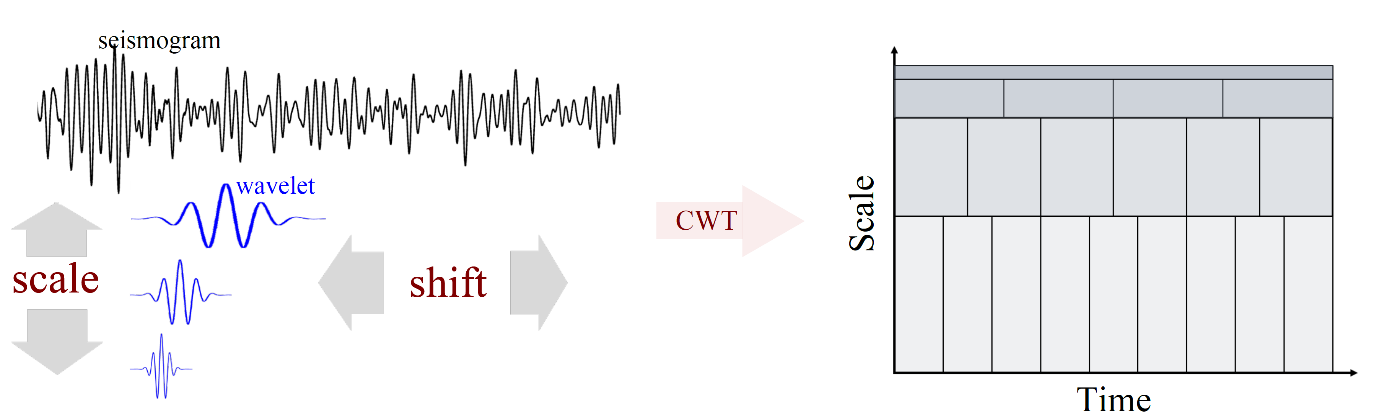
\includegraphics[width=1.0\textwidth,clip=]{figures/cwt_representation.png}
	}
	\caption{Visual representation of CWT.
	}
	\label{F-cwt}
\end{figure}

% MathType!MTEF!2!1!+-
% feaagKart1ev2aaatCvAUfeBSjuyZL2yd9gzLbvyNv2CaerbuLwBLn
% hiov2DGi1BTfMBaeXatLxBI9gBaerbd9wDYLwzYbItLDharqqtubsr
% 4rNCHbGeaGqiVu0Je9sqqrpepC0xbbL8F4rqqrFfpeea0xe9Lq-Jc9
% vqaqpepm0xbba9pwe9Q8fs0-yqaqpepae9pg0FirpepeKkFr0xfr-x
% fr-xb9adbaqaaeGaciGaaiaabeqaamaabaabaaGcbaWaaGbaaeaaca
% qGybWaaeWaaeaacaWGHbGaaiilaiaadkgaaiaawIcacaGLPaaaaSab
% aeqabaGaaGOmaiaabseacaqGGaGaaeyBaiaabggacaqG0bGaaeOCai
% aabMgacaqG4baabaGaae4CaiaabogacaqGHbGaaeiBaiaabwgacaqG
% VaGaae4CaiaabIgacaqGPbGaaeOzaiaabshaaaGccaGL44pacqGH9a
% qpdaWdXbqaamaayaaabaGaamiEamaabmaabaGaamiDaaGaayjkaiaa
% wMcaaaWcbaGaae4CaiaabMgacaqGNbGaaeOBaiaabggacaqGSbaaki
% aawIJ-amaayaaabaGaeqiYdK3aa0baaSqaaiaadggacaGGSaGaamOy
% aaqaaiabgEHiQaaakmaabmaabaGaamiDaaGaayjkaiaawMcaaaWcea
% qabeaacaqGGaGaaeiiaiaabccacaqGGaGaaeikaiaabEhacaqGHbGa
% aeODaiaabwgacaqGSbGaaeyzaiaabshacaqGPaaabaGaaeyyaiaab6
% gacaqGHbGaaeiBaiaabMgacaqGZbGaaeyAaiaab6gacaqGNbGaaeii
% aiaabAgacaqG1bGaaeOBaiaabogacaqG0baaaOGaayjo+dGaaGjbVl
% aadsgacaWG0baaleaacqGHsislcqGHEisPaeaacqGHEisPa0Gaey4k
% Iipaaaa!866A!
\[\underbrace {{\rm{X}}\left( {a,b} \right)}_{\scriptstyle2{\rm{D matrix}}\hfill\atop
	\scriptstyle{\rm{scale/shift}}\hfill} = \int\limits_{ - \infty }^\infty  {\underbrace {x\left( t \right)}_{{\rm{signal}}}\underbrace {\psi _{a,b}^ * \left( t \right)}_{\scriptstyle{\rm{    (wavelet)}}\hfill\atop
		\scriptstyle{\rm{analising funct}}\hfill}\;dt} \]


\color{red}{

Inputs/Variables:
\begin{itemize}
	\item Wavelet Function (scipy.signal.ricker): the reference function wavelet that will be used for finding peaks.
	\item Widths ([1, …, 50]): the widths to transform the wavelet in order to find matches in the signal. (less widths results in more peaks being returned)
	\item Others: see pandas.DataFrame.resample documentation.
\end{itemize}}
\color{black}


\color{black}{
Note: SciPy has several wavelet functions:
\begin{itemize}
	\item Ricker wavelet (scipy.signal.ricker)
	\item Daubechies wavelet (scipy.signal.daub): doesn’t work directly, as CWT applies 2 variables.
	\item Cascade Wavelet (scipy.signal.cascade): 
	\item Morlet wavelet (scipy.signal.morlet): worked, got 145 hits vs 30 for ricker. (widths=[1,…,99])
	\item \color{red}{(Not the Meyer wavelet???)}
\end{itemize}}
\color{black}


\subsection{CWT Routine On Basic Peak Functions} %%%%%%%%%%%%%%
\label{SS-cwt-basic-functions}

The CWT peak detection mechanism can be applied to and 1D time signal, to test the performance this was run on a series of generic peak generating functions including a basic Ricker wavelet, a Gaussian and a sinusoidal signal.


\subsection{CWT Routine On Synthetic Flare Data} %%%%%%%%%%%%%%
\label{SS-cwt-synthetic-data}


\subsection{CWT Routine On GOES XRS Observational Data} %%%%%%%%%%%%%%
\label{SS-cwt-goes-xrs}

The CWT peak detection mechanism was applied to the pre-processed GOES XRS timeseries data (XRSB channel) to determine the x/time peaks that correlate to flares.
For each resulting flare detection the activity of RHESSI (true/False) and GOES peak flare classification was determined.


\subsection{Additional Flare Properties} %%%%%%%%%%%%%%
\label{SS-additional-flare-properties}

Peaktime is the single most ubiquitous flare property that can be derived as a direct result of any peak picking algorithm, but further properties can be considered by making basic assumptions about the background distributions and noise.

\color{red}{
The following is work not yet done on the project:
\subsubsection{Find Start/End Times} %%%%%%%%%%%%%%
\label{SSS-find-start-end-times}
This method finds the local minima before and after the given peak and uses these as the start and end of the flare. This is relatively arbitrary and should be redesigned to be more realistic.

\subsubsection{Total Flare Energy} %%%%%%%%%%%%%%
\label{SSS-total-flare-energy}

Using the start and end times, this uses numerical integration via the trapezoidal rule (using the numpy.trapz method), integrating he XRSA energy over the duration of the flare.
This both rests on the arbitrary decision of start/end times and is limited to only watching over a single frequency. Improvements could be made using the XRSA channel, plus adding further data sources for other frequencies.
}


\section{Analysis of Results}
\label{S-analysis}

The performance of the results from CWT were subjected to a statistical comparison to the GOES HEK and RHESSI HEC flare lists, looking for:

\begin{itemize}
	\item Matching Flares: flares that correlate between CWT detection and flare list populations.
	\item False Positive: flares detected by CWT but not in the reference catalogues.
	\item False Negative: flares not detected by CWT but in the reference catalogues.
\end{itemize}


\begin{figure}    %%%%%%%%%%%%%%%%%% FIGURE 1 
	\centerline{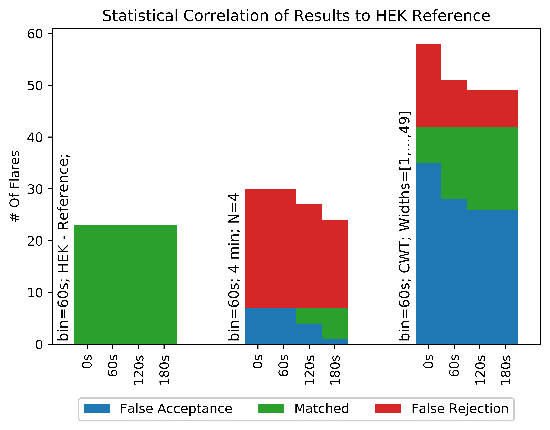
\includegraphics[width=1.0\textwidth,clip=]{figures/results1.png}
	}
	\caption{\color{red}{Fig 2. The graphs of the flare CWT detection population compared to the HEK reference catalogue, with varying window width, for 2012 July 5-6th (left) and 2014 Mar 28-29th (right).}
	}
	\label{F-results1}
\end{figure}





\subsection{} %%%%%%%%%%%%%%
\label{SS-}

\cite{Ryan16}

\subsection{} %%%%%%%%%%%%%%
\label{SS-}

\subsection{} %%%%%%%%%%%%%%
\label{SS-}


\section{}
\label{S-}


\subsection{} %%%%%%%%%%%%%%
\label{SS-}

\subsection{} %%%%%%%%%%%%%%
\label{SS-}

\subsection{} %%%%%%%%%%%%%%
\label{SS-}


\section{}
\label{S-}


\subsection{} %%%%%%%%%%%%%%
\label{SS-}

\subsection{} %%%%%%%%%%%%%%
\label{SS-}

\subsection{} %%%%%%%%%%%%%%
\label{SS-}


\section{}
\label{S-}


\subsection{} %%%%%%%%%%%%%%
\label{SS-}

\subsection{} %%%%%%%%%%%%%%
\label{SS-}

\subsection{} %%%%%%%%%%%%%%
\label{SS-}




\color{red}{
	
\begin{itemize}
	\item 
	\item 
	\item 
	\item 
	\item 
	\item 
\end{itemize}}
\color{black}




   
\section{Conclusion} %%%%%%%%%%%%%%%%%%%%%%%%%%%%%%%%%%%%%%%%
      \label{S-Conclusion} 


%%%%%%%%%%%%%%%%%%%%%%%%%%%%%%%%%%%%%%%%%%%%%%%%%%%%%%%%%%%%%%%%%%%%%%%%%%%
\begin{acks}
 The authors thank ... ({\it note the reduced point size})
\end{acks}

\noindent To change a title use an optional parameter:\par
\verb+\begin{acks}[Acknowledgements]...\end{acks}+



%\acknowledgment US spelling: \verb+\acknowledgment+
%\acknowledgement British  spelling: \verb+\acknowledgement+

%%%%%%%%%%%%%%%%%%%%%%%%%%%%%%%%%%%%%%%%%%%%%%%%%%%%%%%%%%%%%%%%%%%%%%%%%%%
\appendix   


  
%%% BIBLIOGRAPHY %%%%%%%%%%%%%%%%%%%%%%%%%%%%%%%%%%%%%%%%%%%%%%%%%%%%%%%%%%%
     % format of references provided by the journal (.bst)
\bibliographystyle{spr-mp-sola}
     % name your Bibtex file containing your references (.bib)
\bibliography{bibliography}  

     % Checking: look if the file containing the ``\bibitem'' exits
     %           so check if the .bbl file exist (bibTeX compilation)
\IfFileExists{\jobname.bbl}{} {\typeout{}
\typeout{****************************************************}
\typeout{****************************************************}
\typeout{** Please run "bibtex \jobname" to obtain} \typeout{**
the bibliography and then re-run LaTeX} \typeout{** twice to fix
the references !}
\typeout{****************************************************}
\typeout{****************************************************}
\typeout{}}


\end{article} 

\end{document}